\documentclass[spanish,a4paper,12pt,twosides]{book}

%\usepackage[utf8]{inputenc}
\usepackage[T1]{fontenc}
\usepackage[latin1]{inputenc}
\usepackage[margin=1in]{geometry}
%\usepackage{paralist}
\usepackage{graphicx}
\usepackage{url}
\usepackage{times}
\usepackage{babel}
\usepackage{listings}
\usepackage{verbatim}
\usepackage{float}
\usepackage{listings}
\usepackage{color}
\usepackage{array}
\usepackage{fancyvrb}
\usepackage{relsize}
%\usepackage{eurosym}
\usepackage[strict]{chngpage}
\usepackage{qtree}

\pagestyle{headings}

% Some subsvars
\newcommand{\TituloPFC}{Extracci�n de informaci�n de documentos XML mediante
Stanford Parser}
\newcommand{\TituloPFCWeb}{MIEX: Metadata and Information Extractor from small
XML documents}
\newcommand{\AutorPFC}{Ignacio Barrientos Arias}
\newcommand{\Escuela}{Escuela Universitaria de Ingenier�a T�cnica Inform�tica
de Gij�n}
\newcommand{\Universidad}{Universidad de Oviedo}
\newcommand{\Convocatoria}{SEPTIEMBRE 2007}

\newcommand{\sourcepath}
{/home/nacho/devel/pfc/svn/trunk/miex/src/es/uniovi/aic/miex/}
\newcommand{\trunkpath}
{/home/nacho/devel/pfc/svn/trunk/miex/}
\newcommand{\pfctrunkpath}
{/home/nacho/devel/pfc/svn/trunk/doc/pfc}
\newcommand{\codeversion}
{0.1.0}

% Some colour definitions
\definecolor{listinggray}{gray}{0.98}

% Cabeceras
\headheight 15pt

% Listing settings
\lstset
{
	basewidth=0.50em,
	backgroundcolor=\color{listinggray},
	basicstyle=\footnotesize\ttfamily,
	keywordstyle=\bfseries,
	stringstyle=\itshape,
	commentstyle=\itshape,
	showspaces=false,
	showtabs=false,
	showstringspaces=false,
	frame=trbl,
	extendedchars=true,
	%aboveskip=0.5cm,
	%belowskip=0.5cm,
	xleftmargin=0cm,
	xrightmargin=0cm,
	tabsize=1,
	numbers=left, 
	numberstyle=\small,
	stepnumber=5,
	numbersep=5pt
}

% Separation among paragraphs
\parskip  \medskipamount

% Titlesec
\titleformat{\chapter}[frame]
  {\fontfamily{phv}}
  {\filright\large\enspace \chaptertitlename \enspace \thechapter\enspace}
  {8pt}
  {\huge\bfseries\filcenter}
\titleformat{\section}
 {\normalfont\selectfont\large}
 {\thesection}{1em}{\bfseries}[\titlerule]
\titleformat{\section}
  {\fontfamily{phv}\selectfont\Large}
  {\thesection}{1em}{\bfseries}[\titlerule]
\titleformat{\subsection}
  {\fontfamily{phv}\selectfont\large}
  {\thesubsection}{1em}{\bfseries}

% Tweak to dynamically change the margin using a faked environment
\newenvironment{changemargin}[2]{
  \begin{list}{}{
    \setlength{\topsep}{0pt}
    \setlength{\leftmargin}{#1}
    \setlength{\rightmargin}{#2}
    \setlength{\listparindent}{\parindent}
    \setlength{\itemindent}{\parindent}
    \setlength{\parsep}{\parskip}
  }
\item[]}{\end{list}}


% Definici�n de macros para las portadas
\renewcommand{\maketitle}
{
  \begin{titlepage}

  % Portada
	\begin{center}

	\huge\textrm{\textbf{UNIVERSIDAD DE OVIEDO}}\\
	\vspace{1cm}

	\fbox{
\includegraphics[width=3.5cm]{images/uniovi.png}}\\
	\vspace{1cm}

  \Large\textrm{\MakeUppercase{\Escuela}}\\
  \vspace{3cm}

  \Large\textrm{\textbf{PROYECTO FIN DE CARRERA}}\\
  \vspace{2cm}

  \Large\textrm{\textquotedblleft\MakeUppercase{\TituloPFC}\textquotedblright}\\
  \vspace{2cm}

  \Large\textrm{(C�DIGO FUENTE)}\\
  \vspace{1.5cm}

	\Large\textrm{AUTOR:\\ \AutorPFC}\\
	\vspace{0.5cm}
	
	\end{center}
	\begin{flushright}
		\large\textrm{\Convocatoria}
	\end{flushright}

        \pagestyle{empty}
	\cleardoublepage
    
  \end{titlepage}
    
  % Blank page before the main content
  \mbox{}
  \newpage
}


\title{\TituloPFCnorm}
\author{\AutorPFC}
\date{Septiembre de 2007}

\begin{document}

% Arabic page numbers before the main content
\frontmatter

% Crear portadas
\maketitle

%\bibliographystyle{plain}

\chapter*{Resumen}

Documentaci�n del proyecto titulado \emph{\TituloPFC}, 

\section*{Palabras clave}

Recuperaci�n de informaci�n, analizador sint�ctico, analizador sem�ntico,
Stanford Parser, SQL, Java.

\chapter*{Licencia}

El c�digo fuente del programa (disponible en el anexo \ref{sec:source}) se
encuentra licenciado bajo la licencia \emph{GNU General Public License (GPL)}, 
versi�n 2 (anexo \ref{sec:license.gpl}). \\

La documentaci�n se libera bajo la misma licencia que el c�digo fuente del
programa.

\chapter*{Historial de este documento}

\begin{tabular}{|l|l|l|}
 \hline
 \textbf{Fecha} & \textbf{Versi�n} & \textbf{Comentarios} \\\hline
 Jul/2007 & 0.1 & Primer borrador \\\hline
\end{tabular}

\cleardoublepage

\vspace*{10cm}

\begin{flushright}
	\textit{A mi familia y amigos...}
\end{flushright}




\tableofcontents

\newpage

\listoffigures

\newpage

\listoftables

\newpage

% Main stuff
\mainmatter

\chapter{Introducci�n}\label{cap:introduccion}

\section{T�tulo del proyecto}

Si bien el t�tulo original del proyecto es \textit{MIEX: Metadata and
Information Extractor from small XML documents}, para la distribuci�n en el
marco universitario se ha optado por el siguiente t�tulo:

\emph{\TituloPFC}.

\chapter*{Alcance de este documento}

Este libro contiene la documentaci�n del proyecto titulado \emph{\TituloPFC} y
pretende explicar lo m�s breve y concisamente posible como se ha desarrollado
as� como dar las claves necesarias para utilizarlo.

Adem�s de una peque�a memoria que abarcar� los aspectos no t�cnicos y el
historial del proceso de desarrollo, se incluye un cap�tulo completo destinado
a personal t�cnico (principalmente desarrolladores), un manual para
usuarios finales y un peque�o ep�grafe destinado a experimentaci�n.

\section*{Palabras clave}

Recuperaci�n de informaci�n, analizador sint�ctico, analizador sem�ntico,
Stanford Parser, SQL, Java.

\section*{Aclaraci�n sobre el t�tulo}

Aunque el t�tulo del proyecto escogido para la distribuci�n y utilizaci�n en el
marco universitario es \textit{\TituloPFC}, el t�tulo original
es \textbf{\TituloPFCWeb}, por lo que, a lo largo de este documento, se har�
referencia al proyecto utilizando los dos t�tulos indistintamente.

\section*{Historial}

\begin{center}
\begin{tabular}{rcl}
 \hline \hline
 \multicolumn{1}{c}{\textbf{Fecha}} &
 \multicolumn{1}{c}{\textbf{Versi�n}} &
 \multicolumn{1}{c}{\textbf{Comentarios}} \\
 \hline \hline
 25/06/07 & 0.1 & Primer borrador para revisi�n.\\
 \hline
 19/07/07 & 0.2 & Segundo borrador para revisi�n.\\
 \hline
 09/08/07 & 0.3 & Tercer borrador para revisi�n.\\
 \hline
 nn/07/07 & 1.0 & Primera versi�n para publicaci�n.\\
 \hline \hline
\end{tabular}
\end{center}

\section{Primeros pasos}

La importancia que posee la recuperaci�n de informaci�n es vital en nuestros
d�as. A partir de un cierto volumen de texto se hace imprescindible un
sistema organizativo que posibilite la localizaci�n de la informaci�n que se
precise en cualquier momento. Como es de suponer, para construir los
citados sistemas organizativos es necesario el an�lisis previo, tanto sint�ctico
como sem�ntico, de los textos.

En general, los analizadores de lenguaje natural existentes tienen varias
desventajas. Una de ellas, es que no poseen interfaces que hagan f�cil su manejo
y por tanto hacen perder mucho tiempo al usuario en escribir c�digo adicional o
en leerse mucha documentaci�n para utilizarlos. Por otro lado, no suelen
proporcionar mecanismos para guardar la informaci�n extra�da en medios flexibles
para posteriores consultas.

El objetivo de este proyecto es la elaboraci�n de un envoltorio
(\textit{wrapper}) de uno de los analizadores m�s conocidos, el Stanford
Parser. Con �ste envoltorio se pretende hacer que el manejo del mismo sea lo
m�s sencillo posible, para que, la persona que lo use, se pueda abstraer
totalmente del funcionamiento interno del software y poder analizar documentos
f�cilmente. Para paliar la segunda desventaja de estos analizadores, se
proporcionar� un sistema para el almacenamiento de la informaci�n en una base
de datos relacional.

Es importante que el usuario de este proyecto tenga en cuenta que las
capacidades de an�lisis tanto sem�ntico como sint�ctico est�n restringidas a las
propias limitaciones del analizador base que se toma, por lo que se aconseja
encarecidamente leer documentaci�n sobre el Stanford Parser antes de continuar
con este libro.

Si lo que quiere es aprender directamente como utilizar MIEX, le aconsejo que
lea directamente al cap�tulo \ref{cap:manual}, donde se explica como ponerlo
en marcha. Si prefiere conocer el formato de las colecciones a analizar o la
informaci�n que se extrae de las mismas, siga leyendo este ep�grafe.






\section{Objetivos}

Entre otras caracter�sticas, el principal objetivo de MIEX es analizar
sint�cticamente colecciones de peque�os documentos escritos en ingl�s. En el
siguiente cap�tulo se ver� con m�s profundidad el funcionamiento interno, pero
si por ahora nos abstraemos, lo primero deber�a de ser separar cada documento
en oraciones y posteriormente analizarlas.

Se realizan dos tipos de an�lisis, a nivel de palabra individual, y a nivel de
relaciones entre palabras, vamos a ver un ejemplo. Veamos que an�lisis produce
el analizador para la siguiente oraci�n.

\textit{The Debian Project is an association of individuals.}

La representaci�n m�s vistosa del resultado es en forma de �rbol, por lo que lo
dibujaremos as�. Para saber el significado de cada etiqueta no tiene m�s que
echar un vistazo al anexo \ref{sec:penntags}.

\Tree[.ROOT [.S [.NP [.DT The ] [.NNP Debian ] [.NNP Project ] ] [.VP [.VBZ is
] [.NP [.NP [.DT an ] [.NN association ] ] [.PP [.IN of ] [.NP [.NNS individuals
 ] ] ] ] ] ] ]
 

Se puede ver que se asignan etiquetas a nivel de palabra, a nivel de grupo
frasal y a nivel clausal, tal y como se hace habitualmente en cualquier an�lisis
sint�ctico.

Aprovecharemos tambi�n que el analizador calcula las dependencias entra
palabras:

\begin{Verbatim}[fontsize=\relsize{-1}]
det(Project-3, The-1)
nn(Project-3, Debian-2)
nsubj(association-6, Project-3)
cop(association-6, is-4)
det(association-6, an-5)
prep_of(association-6, individuals-8)
\end{Verbatim}

Tanto el an�lisis a nivel de palabra (y obviamente a nivel de grupo) como las
relaciones entre las palabras ser� la informaci�n que nos va a interesar
guardar.

En resumen, una buena visi�n global de los objetivos de MIEX es la siguientes:

\begin{itemize}
	\item Comprobaci�n de integridad y an�lisis de documentos XML.
	\item Uso del Stanford Parser para extraer los an�lisis
sint�cticos de las oraciones as� como las relaciones entre las palabras.
	\item An�lisis y limpieza de la informaci�n recabada.
	\item Almacenamiento en un medio flexible para posteriormente realizar
consultas a medida.
\end{itemize}


\begin{figure}[h]
\begin{center}
	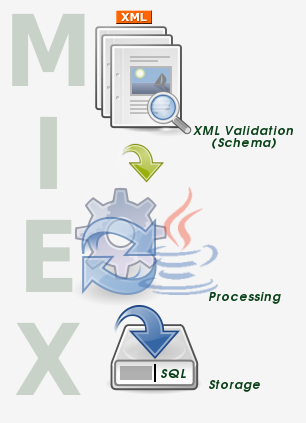
\includegraphics[bb=0 0 148 240]{images/miex.png}
	% miex.png: 257x416 pixel, 125dpi, 5.22x8.45 cm, bb=0 0 148 240
\end{center}
\caption{Esquema de funcionamiento de MIEX}
\end{figure} 


\section{Formato de los ficheros a tratar}

En la siguiente secci�n se explicar�n todos los aspectos relevantes a los
ficheros de entrada que procesar� MIEX.

Los ficheros de entrada con los que va a interactuar MIEX est�n todos en
formato XML, lo cual facilita el tratamiento y an�lisis del contenido.

\subsection{�Qu� es XML?}

XML\footnote{http://es.wikipedia.org/wiki/XML}, sigla en ingl�s de eXtensible
Markup Language (�lenguaje de marcas extensible�), es un metalenguaje extensible
de etiquetas desarrollado por el World Wide Web Consortium (W3C). Es una
simplificaci�n y adaptaci�n del SGML y permite definir la gram�tica de lenguajes
espec�ficos (de la misma manera que HTML es a su vez un lenguaje definido por
SGML). Por lo tanto XML no es realmente un lenguaje en particular, sino una
manera de definir lenguajes para diferentes necesidades.

\subsection{El lenguaje utilizado}\label{sec:schema}

El lenguaje que se define utilizando XML para representar las colecciones
satisface la siguiente plantilla (concepto m�s conocido por su nombre
en ingl�s, \textit{XML Schema}).

\begin{Verbatim}[label=default.xsd, frame=single,framesep=2pt,fontsize=\relsize{
-1 } ]
<?xml version="1.0"?>
<xs:schema xmlns:xs="http://www.w3.org/2001/XMLSchema">

<xs:complexType name="categoriestype">
 <xs:sequence>
  <xs:element name="D" type="xs:string" minOccurs="1" 
   maxOccurs="unbounded"/>
 </xs:sequence>
</xs:complexType>

<xs:complexType name="doctype">
  <xs:all>
   <xs:element name="TOPIC" type="categoriestype" minOccurs="1" 
    maxOccurs="1"/>
   <xs:element name="TITLE" type="xs:string" maxOccurs="1"/>
   <xs:element name="BODY" type="xs:string" minOccurs="1" 
    maxOccurs="1"/>
  </xs:all>
</xs:complexType>

<xs:element name="COLLECTION">
<xs:complexType>
 <xs:sequence>
  <xs:element name="DOCTRAIN" type="doctype"
    minOccurs="0" maxOccurs="unbounded"/>
  <xs:element name="DOCTEST" type="doctype" minOccurs="0"
    maxOccurs="unbounded"/>
 </xs:sequence>
</xs:complexType>
</xs:element>

</xs:schema>
\end{Verbatim}

Por lo que cada fichero que represente una colecci�n de documentos ser�
gen�ricamente de esta forma:

\begin{Verbatim}[frame=single,framesep=2pt,fontsize=\relsize{-1}]
<collection>
 <doctrain>
 <topic> <d>c1</d> <d>c2</d> ... <d>cn</d> </topic>
 <title>un t�tulo</title>
 <body>un cuerpo</body>
 </doctrain>
 ...
 <doctrain>
 <topic> <d>c1</d> <d>c2</d> ... <d>cn</d> </topic>
 <title>otro t�tulo</title>
 <body>otro cuerpo</body>
 </doctrain>
</collection>
 \end{Verbatim}
 
\subsection{�Qu� informaci�n es importante?}

De cara a analizar el contenido es importante la informaci�n comprendida en las
etiquetas \textit{title} y \textit{body}. Por otro lado, las categor�as de cada
documento tambi�n tienen importancia, ya que en un futuro podr�a ser interesante
analizar la informaci�n obtenida en funci�n a la categor�a, por ejemplo, para
hacer agrupamientos de palabras.

\subsection{Ejemplo de una colecci�n}

A continuaci�n, un peque�o ejemplo de un fichero de colecci�n llamado
\textit{computers.xml}.

\begin{Verbatim}[label=computers.xml,frame=single,framesep=2pt,fontsize=\relsize
{
-1}]
<collection>
 <doctrain>
 <topic> <d>debian</d> <d>linux</d> <d>OS</d> </topic>
 <title>Debian project</title>
 <body> Debian is a free operating system (OS) for your computer. An 
 operating system is the set of basic programs and utilities that 
 make your computer run. Debian uses the Linux kernel (the core of 
 an operating system), but most of the basic OS tools come from the 
 GNU project; hence the name GNU/Linux.
 </body>
 </doctrain>
 <doctrain>
 <topic> <d>computing</d> <d>search</d> <d>engine</d> </topic>
 <title>Google</title>
 <body> Google Inc. (NASDAQ: GOOG and LSE: GGEA) is an American 
 public corporation, specializing in Internet search and online 
 advertising. The company had 10,674 full-time employees as of 
 December 31, 2006, and is based in Mountain View, California. 
 </body>
 </doctrain>
</collection>
\end{Verbatim}

Se puede apreciar que se trata de una colecci�n formada por dos documentos
titulados \textit{Debian project} y \textit{Google}. El primer documento se
encuentra en las categor�as \textit{debian}, \textit{linux} y \textit{OS} as�
como el segundo est� en las categor�as \textit{computing}, \textit{search}
y \textit{engine}.

\subsection{Adaptando ficheros mal formados}

Los ficheros de colecci�n para los que inicialmente fue dise�ado MIEX no ten�an
un formato correcto, concretamente el XML no inclu�a nodo ra�z ni cerraba
correctamente las etiquetas. Para paliar este problema, se han desarrollado un
par de herramientas que permiten f�cilmente la adaptaci�n al formato correcto
de los ficheros problem�ticos. Se proporcionar� m�s informaci�n en los
siguientes cap�tulos.


\section{Almacenamiento de la informaci�n}

A la hora de decidir el medio para almacenar los resultados obtenidos
r�pidamente se descart� la opci�n de utilizar ficheros de texto plano, ya que
requerir�an la construcci�n de analizadores adicionales para, una vez se
quiera consultar los resultados, poder recuperar la informaci�n.

Finalmente se decidi� utilizar una base de datos relacional para poder, en
cierta manera, dise�ar una estructura lo m�s c�moda posible para dejar abierto
un gran abanico de posibilidades a la hora de consultar la informaci�n obtenida.

En el cap�tulo que se dedica a los aspectos t�cnicos, se explica la base de
datos utilizada as� como la estructura de la misma. 

\section{Recursos sobre el proyecto}

\subsection{P�gina web}

Una vez sea presentado el proyecto mi intenci�n es seguir desarrollando
MIEX en mis ratos libres. Para hacer el trabajo m�s transparente, existe un
proyecto creado en SourceForge\footnote{http://www.sourceforge.net} as� como una
p�gina web en la siguiente direcci�n.

\url{http://miex.sf.net}

A trav�s de esa URI es posible obtener la informaci�n m�s actualizada acerca de
MIEX, estar a d�a de los eventos que rodean al proyecto y obtener
\textit{snapshots} actualizadas del c�digo fuente.

\subsection{RSS}

Si desea suscribirse al canal RSS\footnote{http://es.wikipedia.org/wiki/RSS} que
contiene las noticias no tiene m�s que a�adir la siguiente direcci�n en su
agregador favorito:

\url{http://sourceforge.net/export/rss2_projnews.php?group_id=187602}

\subsection{Subversion}

El repositorio donde se lleva el control de las versiones del c�digo fuente
(utilizando Subversion\footnote{http://subversion.tigris.org/}) se
encuentra en \url{https://miex.svn.sourceforge.net/svnroot/miex} y tiene la
siguiente estructura:

\begin{itemize}
	\item \textbf{branches} - Ramas de desarrollo paralelas a
\textit{trunk}
	\item \textbf{tags} - Versiones congeladas (releases)
	\item \textbf{trunk} - Rama principal de desarrollo de MIEX 
	\begin{itemize}
		\item \textbf{doc} - Documentaci�n (presentaciones, libros...)
		\item \textbf{miex} - C�digo fuente del proyecto
		\item \textbf{web} - P�gina web
	\end{itemize}
\end{itemize}

\textbf{Nota:} Use el contenido de \textit{trunk} con precauci�n. Debido a que
es c�digo que suele cambiar con mucha frecuencia, puede descargar una captura
inestable y obtener resultados inesperados. Si desea una versi�n estable y
funcional desc�rgela directamente de la p�gina web o obt�ngala desde
\textit{tags}.



\section{El proceso de desarrollo}

Aproximadamente, la siguiente tabla (\ref{tab:proceso-dev}) recoge el tiempo
dedicado a cada una de las tareas llevadas a cabo durante el desarrollo del
proyecto.

\begin{table}[h]
\begin{center}
\begin{tabular}{lcl}
 \hline \hline
 \multicolumn{1}{c}{\textbf{Tarea}} &
 \multicolumn{1}{c}{\textbf{Fecha de comienzo}} &
 \multicolumn{1}{c}{\textbf{Tiempo \small{(d�as)}}} \\
 \hline \hline
 Estudio de viabilidad & 07/12/06 & 15\\
 \hline
 An�lisis y dise�o & 08/01/07 & 40\\
 \hline
 Desarrollo del software & 25/02/07 & 140\\
 \hline
 Elaboraci�n de la documentaci�n & 11/06/07 & 30\\
 \hline \hline
\end{tabular}
\caption{Tiempo de dedicaci�n a cada tarea}
\label{tab:proceso-dev}
\end{center}
\end{table}

En el gr�fico de la figura \ref{fig:svn-act} se muestra la actividad del
repositorio de c�digo y documentaci�n durante los �ltimos doce meses.

\begin{figure}[h]
\begin{center}
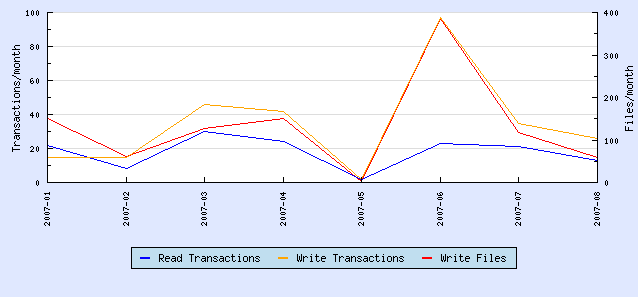
\includegraphics[scale=0.8]{images/svn-activity.png}
\end{center}
\caption[Gr�fico de actividad en el repositorio de c�digo y
documetantaci�n]{Gr�fico de actividad en el repositorio SVN (SourceForge.net)}
\label{fig:svn-act}
\end{figure}

\newpage





\chapter{Metodolog�a}

%\input{metodologia/rup.tex}

%\input{metodologia/concepcion.tex}

%\input{metodologia/sad.tex}

%\input{metodologia/construccion.tex}


\chapter{Manual de usuario}

%\input{manuales/tecnico.tex}

%\input{manuales/despliegue.tex}

%\input{manuales/usuario.tex}



\section{Conclusiones}

Por la parte acad�mica, este proyecto me ha servido para tener un primer
contacto con el mundo de la recuperaci�n de informaci�n y el an�lisis de
lenguaje natural.

En los aspectos t�cnicos, el desarrollo me ha ayudado a practicar con Java, y a
refrescar mis conocimientos de \LaTeX. Aunque me he ayudado de un conjunto de
libros \cite{IntroLaTeX} \cite{LaTeXimprenta} y \cite{LearningJava}, la ayuda
m�s significativa la he obtenido de diversas p�ginas web, recogidas en
el ap�ndice \ref{cha:referencias}. Respecto a el Stanford Parser, como se puede
observar en el cap�tulo \ref{cap:experimentacion}, es posible concluir que el
rendimiento del analizador es aceptable, incluso con oraciones de tama�o
considerable. De todos modos, no me es posible realizar una comparaci�n con
otros analizadores similares ya que utilizar el Stanford Parser era un requisito
invariable desde el comienzo el proyecto.

En lo personal, estando acostumbrado al trabajo en grupo en diversos proyectos,
me he dado cuenta de lo aburrido que puede llegar a ser trabajar de
manera individual. Esta falta de compa�eros no se nota tanto cuando se realizan
tareas divertidas, como el desarrollo del software, pero si a la hora de hacer
tareas m�s pesadas, como escribir documentaci�n.

No me extiendo m�s, si quiere saber m�s cosas si�ntase libre de preguntarme
mediante correo electr�nico\footnote{mailto:nacho@criptonita.com}



\appendix


%
\chapter{Propuesta inicial\label{sec:propuesta}}

Diego Berrueta (Agosto 2005)

Las listas de correo son parte fundamental de la comunicación en Internet.
Existen listas de correo dedicadas a cualquier tema de inter\'es imaginable.
Hoy en día, es común que las listas de correo publiquen sus archivos (los
mensajes antiguos) en forma de páginas web, lo que dispara su utilidad,
especialmente en combinación con los buscadores actuales. Gracias a esta 
publicación, es posible consultar los mensajes desde el navegador, sin 
necesidad de estar suscrito a las listas de correo, y también se puede 
localizar un mensaje usando Google u otro buscador.

Estos archivos contienen una formidable base de conocimiento, especialmente
en temas técnicos. Un uso muy común consiste en introducir un mensaje de error 
(de una aplicación) en Google\footnote{\url{http://www.google.es/}} y obtener 
como resultado un mensaje archivado que aborda el problema, probablemente 
porque alguien se ha encontrado previamente con el mismo error y ha efectuado 
la consulta en una lista de correo pública. Con suerte, alguna de las respuestas 
al mensaje localizado contendrá la solución al problema, aportada por un experto 
suscrito a la lista de correo.

\section*{Problemas}

Por desgracia, consultar los archivos de una lista de correo en la web es
más incómodo que hacerlo mediante un cliente de correo electrónico.
Por poner sólo algunos ejemplos, el navegador no permite ejecutar ninguna
de estas acciones:

\begin{itemize}
 \item Mostrar el hilo de la conversación en forma de árbol.
 \item Imprimir el hilo completo.
 \item Mostrar una lista de los mensajes entre dos fechas arbitrarias.
 \item Ocultar los mensajes que no tienen respuestas.
 \item Mostrar sólo los mensajes de una cierta persona.
 \item Buscar una cadena de texto sólo en los mensajes de un determinado hilo.
 \item Descargar el hilo como un fichero, o cualquier otra forma de exportar la
 información para poder acceder a ella desde un cliente de correo electrónico
 o fuera de línea.
 \item Responder a un mensaje usando un cliente de correo (o un webmail) y 
 citando el mensaje original.
\end{itemize}

Al indexar los archivos de las listas de correo, los buscadores se encuentran
en ocasiones que los mensajes están replicados en varios servidores (mirrors).
Al no tener forma de identificar los mensajes, la desgraciada consecuencia
es que los mensajes aparecen varias veces en los resultados de las búsquedas,
y sólo el usuario puede darse cuenta de que se trata de una repetición.
Naturalmente, el comportamiento ideal sería que los mensajes aparecieran
sólo una vez en los resultados del buscador.

\section*{Origen de los problemas: pérdida de información}

En el origen de estos problemas se encuentra una pérdida de información
que se produce al convertir los mensajes archivados a HTML para su publicación
en la web.

Los gestores más habituales de listas de correo (mailman, majordomo, sympa,
etc.) generan un fichero en formato Mailbox (mbox) con los mensajes que
han sido enviados a la lista.

Otros programas independientes, como hypermail, monharc, pipermail..., se
especializan en convertir el fichero Mailbox en un conjunto de páginas
web estáticas.

Los programas más sofisticados son capaces de generar índices complejos
de los archivos (por fecha, por autor, por hilo...), con múltiples referencias
cruzadas entre los mensajes en forma de hipervínculos (mensaje anterior,
mensaje siguiente, etc.).

Pero incluso en el mejor de los casos, esta información sólo es comprensible
para el usuario, nunca para la máquina.

En consecuencia, es imposible explotarla más allá de las formas previstas
por el programa que ha generado los archivos.

Entre la información que se pierde en la publicación, se encuentra:

\begin{itemize}
 \item El asunto del mensaje.
 \item El autor del mensaje.
 \item La fecha del mensaje.
 \item La referencia a la lista de correo en la que se publicó el mensaje.
 \item La referencia al mensaje anterior, si existe.
 \item Las referencias (enlaces) a las posibles respuestas al mensaje.
\end{itemize}

\section*{Propuesta para conservar la información}

Las tecnologías de la web semántica (y concretamente, RDF) son perfectamente
capaces de publicar en la web toda la información señalada en la sección
anterior. Dado que la información ya existe en el origen, no es necesario 
ningún procedimiento manual para enriquecerla. Tan sólo debe considerarse un 
proceso de conversión que no desprecie la información, sino que la publique 
junto con los archivos en HTML. De esta forma, las listas de correo se 
introducirían en la web semántica.

\section*{Aplicaciones}

Enriquecer semánticamente la publicación web de los archivos de las listas
de correo abriría la puerta a nuevas aplicaciones:

\begin{itemize}
  \item Eliminar la aparición repetida de los mismos mensajes en los resultados
 	de los buscadores. Para lograrlo, los buscadores deberían procesar la 
	información semántica para reconocer las copias (mirrors) de los archivos.
  \item Implementar en los navegadores nuevas funcionalidades para resolver alguno
	de los problemas antes señalados. Estas capacidades, que mejorarían 
	sensiblemente la comodidad en la consulta de los archivos, podrían añadirse 
	como extensiones o plug-ins de los navegadores actuales.
  \item Obtener información sobre los suscriptores de una lista de correo. Por 
	ejemplo, conocer en qué otras listas de correo participa una persona. 
	Esta aplicación es especialmente interesante en conexión con 
	FOAF\footnote{\url{http://www.foaf-project.org/}.} De este modo, se 
	podría sacar una \emph{orla} con las fotos de los participantes en una 
	lista de correo\footnote{Como hace GNOME, véase 
	\url{http://planet.gnome.org/heads/}}, o situarlos geográficamente en un 
	mapa\footnote{Como hace Debian, 
	véase \url{http://www.debian.org/devel/developers.loc}}.
  \item Facilitar la internacionalización. Al hacer comprensibles las relaciones entre 
	los mensajes por el software, el navegador proporcionaría las opciones de 
	exploración (mensaje siguiente, mensaje anterior, etc.) en el idioma del 
	usuario, independientemente del idioma en el que se encontrasen las páginas 
	HTML.
  \item Mejorar la accesibilidad de la información. Las tecnologías de accesibilidad 
	podrían informar sobre quién es el autor del mensaje o cuántas respuestas hay, 
	usando la voz u otros medios.
\end{itemize}

\section*{Estado del arte}

Existen algunos trabajos similares a esta propuesta:

\begin{itemize}
  \item El proyecto DOAML\footnote{\url{http://www.doaml.net/}} consiste en un 
	vocabulario RDF para describir listas de correo. Como ejemplo, en 
	la web del proyecto se encuentran las descripciones de las listas 
	de correo del W3C. La información de este vocabulario limita sus 
	referencias a los mensajes archivados a un enlace a la versión HTML 
	de éstos.
  \item Por otro lado, EMiR\footnote{\url{http://xmlns.filsa.org/emir/}} es un 
	esquema RDF para describir mensajes de correo electrónico. 
  \item En la misma línea se encuentra XMTP\footnote{\url{http://www.openhealth.org/xmtp/}}.
\end{itemize}

\section*{Conclusiones}

Introducir los archivos de las listas de correo en la web semántica sólo
requiere disponer de una aplicación de publicación que utilice la tecnología
apropiada (RDF) como complemento al HTML.

Con un mínimo esfuerzo, los administradores de todas las listas de correo
podrían emplear la aplicación en sus listas, por lo que la implantación
sería rápida\footnote{En realidad, cualquier suscriptor (no necesariamente 
el administrador) de una lista de correo podría publicar los archivos enriquecidos.
Tan sólo debería disponer de todos los mensajes antiguos almacenados en su 
cliente de correo electrónico, y exportarlos al formato Mbox.}. Además, al 
no requerirse la participación de un experto para el enriquecimiento de la 
información, resultaría posible enriquecer inmediatamente grandes volúmenes 
de información, incluso listas de correo que lleven muchos años en funcionamiento.

El desarrollo de una aplicación de estas características requeriría, en
primer lugar, la creación de un esquema de información, que muy bien podría
ser una combinación de los ya existentes; y en segundo lugar, el procesamiento 
de un fichero Mbox para extraer la información que contiene.


\chapter{C�digo fuente\label{sec:source}} 

La versi�n actual del c�digo (versi�n \codeversion) se incluye en este
ep�grafe. De cara a poner el software en producci�n se aconseja obtener la
�ltima versi�n de la p�gina web del proyecto\footnote{http://miex.sf.net}

\section*{Paquete Config}

\subsection*{ConfigCMDLine.java}

\lstinputlisting[language=Java]{\sourcepath/config/ConfigCMDLine.java}

\subsection*{ConfigFile.java}

\lstinputlisting[language=Java]{\sourcepath/config/ConfigFile.java}

\section*{Paquete Datastr}

\subsection*{ExtendedTaggedWord.java}
\lstinputlisting[language=Java]{\sourcepath/datastr/ExtendedTaggedWord.java}

\subsection*{MyCategories.java}
\lstinputlisting[language=Java]{\sourcepath/datastr/MyCategories.java}

\subsection*{MyCollection.java}
\lstinputlisting[language=Java]{\sourcepath/datastr/MyCollection.java}

\subsection*{MyDoc.java}
\lstinputlisting[language=Java]{\sourcepath/datastr/MyDoc.java}

\section*{Paquete filter}

\subsection*{GlobalFilter.java}
\lstinputlisting[language=Java]{\sourcepath/filter/GlobalFilter.java}

\subsection*{NumbersDetector.java}
\lstinputlisting[language=Java]{\sourcepath/filter/NumbersDetector.java}

\subsection*{Porter.java}
\lstinputlisting[language=Java]{\sourcepath/filter/Porter.java}

\subsection*{StopWordsDetector.java}
\lstinputlisting[language=Java]{\sourcepath/filter/StopWordsDetector.java}

\subsection*{UselessTagsDetector.java}
\lstinputlisting[language=Java]{\sourcepath/filter/UselessTagsDetector.java}

\section*{Paquete Input}

\subsection*{FieldsParser.java}
\lstinputlisting[language=Java]{\sourcepath/input/FieldsParser.java}

\subsection*{SAXCollectionUnmarshaller.java}
\lstinputlisting[language=Java]{\sourcepath/input/SAXCollectionUnmarshaller.java
}

\subsection*{XMLValidator.java}
\lstinputlisting[language=Java]{\sourcepath/input/XMLValidator.java}

\section*{Paquete Run}

\subsection*{Miex.java}
\lstinputlisting[language=Java]{\sourcepath/run/Miex.java}

\section*{Paquete Semantic}

\subsection*{Extractor.java}
\lstinputlisting[language=Java]{\sourcepath/semantic/Extractor.java}

\section*{Paquete Sql}

\subsection*{SQLHandler.java}
\lstinputlisting[language=Java]{\sourcepath/sql/SQLHandler.java}

\section*{Paquete Tools}

\subsection*{HexString.java}
\lstinputlisting[language=Java]{\sourcepath/tools/HexString.java}

\subsection*{MD5.java}
\lstinputlisting[language=Java]{\sourcepath/tools/MD5.java}

\section*{Otros}

\subsection*{Makefile (MIEX)}
\lstinputlisting{\trunkpath/Makefile}

\subsection*{Build.xml (MIEX)}
\lstinputlisting{\trunkpath/build.xml}

\subsection*{Makefile (Documentaci�n)}
\lstinputlisting{Makefile}


%
\chapter{Citas al proyecto}

\section{Carta de reconocimiento de John Breslin}

El Dr. John Breslin\footnote{\url{http://www.deri.ie/about/team/member/john_breslin/}},
líder del subcluster de software social de Deri Galway\footnote{\url{http://www.deri.ie/}},
el 29 de Noviembre de 2006 ha tenido la amabilidad de dedicar estas alentadoras palabras 
al proyecto:

\begin{quote}
 The SWAML project fulfills a much-needed requirement for the Semantic 
 Web: to be able to refer to semantic versions of email messages and 
 their properties using a resource URI.  I am delighted that the SWAML 
 group have decided to use our SIOC vocabulary for their work, especially 
 now as SIOC is beginning to achieve traction in terms of both metadata 
 creation and applications that can make use of this metadata.  By 
 reusing the SIOC vocabulary for describing online discussions, SWAML 
 allows users of SIOC to refer to email messages from other discussions 
 taking place on forums, blogs, etc., so that distributed conversations 
 can occur across these discussion media.  Also, by providing email 
 messages in SIOC format, SWAML are providing a rich source of data, 
 namely mailing lists, for use in SIOC applications.  I am also happy to 
 see the SWAML creators developing their own applications that will work 
 with SIOC data - the Buxon sioc:Forum visor is a great example of a 
 program using SIOC message data that can come from one or many sources 
 (e.g. from a virtual forum or container of posts from multiple sites 
 and systems).
\end{quote}

\newpage

\section{Citas en blogs}

El modelo de desarrollo abierto y colaborativo ha conseguido que el proyecto haya 
entrado de manera natural en la comunidad científica que trabaja en el campo de la
Web Semántica. Esto ha hecho que dicha comunidad haya seguido con interés los avances 
en el proyecto, coleccionando un puñado de citas que siempre son de agradecer:

\subsection*{SIOC News\footnote{\url{http://apassant.net/blog/post/2006/10/01/117-sioc-news}}}

Por Alexandre Passant el domingo 1 de Octubre de 2006, día previo al lanzamiento 
de la primera versión de SWAML:

\begin{quote}
 (...) Wikier mentionned on \#sioc that SWAML, a project he's involved in to translate mailing 
 lists in RDF, will use SIOC. (...)
\end{quote}

\subsection*{State of the SIOC-o-sphere\footnote{\url{http://www.johnbreslin.com/blog/2006/11/07/state-of-the-sioc-o-sphere-number-3/}}}

Por John Breslin el martes 7 de Noviembre de 2006, después de la publicación de Buxon:

\begin{quote}
 (...) SWAML, the Semantic Web Archive of Mailing Lists, is now using SIOC as its base 
 ontology. Last week, the developers also announced that SWAML now incorporates Buxon, a sioc:Forum 
 visor written in PyGTK (see screenshot). Excellent stuff  (...)
\end{quote}

\subsection*{Buxon visor for sioc:Forum browsing\footnote{\url{http://www.johnbreslin.com/blog/2006/11/08/buxon-visor-for-siocforum-browsing/}}}

Por John Breslin el miércoles 8 de Noviembre de 2006, dando su impresión de Buxon:

\begin{quote}
 I've been testing out the Buxon visor for browsing SIOC forums, created by the SWAML 
 developers and written in PyGTK.

 So far, it works great (with SWAML-generated data). I used an example script packaged 
 with python-libgmail (archive.py) to download an inbox from a GMail account (subscribed 
 to the sioc-dev mailing list) to mbox format, and then ran swaml.py on that mbox to 
 convert it to SIOC RDF. The resulting RDF is here, and I successfully browsed this with 
 Buxon. Great job, SWAML guys!

 This is a nice demonstrator, and it just remains to do the same for a few more 
 SW-related mailing lists...
\end{quote}

\section{Otras citas}

\subsubsection*{nice phone from Patrick\footnote{\url{http://flickr.com/photos/leobard/294518500/in/pool-iswc/}}}

Uldis Bojars comentó\footnote{\url{http://groups.google.com/group/sioc-dev/browse_thread/thread/c9689c4762390396/674fa1a9fedfc1ac}}
en la lista de correo de SIOC-Dev la foto que habían hecho en el
ISWC2006\footnote{\url{http://iswc2006.semanticweb.org/}} con 
PlanetRDF\footnote{\url{http://planetrdf.com/}} visto desde un móvil. Con la casualidad,
como se puede ver en la figura~\ref{fig:planetrdf-mobile}, que el post que en ese momento 
estaba en portada era el de John Breslin hablando de Buxon.

\begin{figure}[ht]
	\centering
	\includegraphics{images/screenshots/planetrdf-mobile.png}
	\caption{PlanetRDF visto desde un móvil con un post hablando de Buxon}
	\label{fig:planetrdf-mobile}
\end{figure}





\chapter{Licencias} 

\section{GNU General Public License (GPL)\label{sec:license.gpl}}

\begin{center}
{\parindent 0in

Version 2, June 1991

Copyright \copyright\ 1989, 1991 Free Software Foundation, Inc.

\bigskip

51 Franklin St, Fifth Floor, Boston, MA  02110-1301, USA

\bigskip

Everyone is permitted to copy and distribute verbatim copies
of this license document, but changing it is not allowed.

\bigskip

\url{http://www.gnu.org/licenses/gpl.html}
}
\end{center}

\bigskip

\begin{center}
 {\Large \sc Preamble}
\end{center}

The licenses for most software are designed to take away your freedom to
share and change it.  By contrast, the GNU General Public License is
intended to guarantee your freedom to share and change free software---to
make sure the software is free for all its users.  This General Public
License applies to most of the Free Software Foundation's software and to
any other program whose authors commit to using it.  (Some other Free
Software Foundation software is covered by the GNU Library General Public
License instead.)  You can apply it to your programs, too.

When we speak of free software, we are referring to freedom, not price.
Our General Public Licenses are designed to make sure that you have the
freedom to distribute copies of free software (and charge for this service
if you wish), that you receive source code or can get it if you want it,
that you can change the software or use pieces of it in new free programs;
and that you know you can do these things.

To protect your rights, we need to make restrictions that forbid anyone to
deny you these rights or to ask you to surrender the rights.  These
restrictions translate to certain responsibilities for you if you
distribute copies of the software, or if you modify it.

For example, if you distribute copies of such a program, whether gratis or
for a fee, you must give the recipients all the rights that you have.  You
must make sure that they, too, receive or can get the source code.  And
you must show them these terms so they know their rights.

We protect your rights with two steps: (1) copyright the software, and (2)
offer you this license which gives you legal permission to copy,
distribute and/or modify the software.

Also, for each author's protection and ours, we want to make certain that
everyone understands that there is no warranty for this free software.  If
the software is modified by someone else and passed on, we want its
recipients to know that what they have is not the original, so that any
problems introduced by others will not reflect on the original authors'
reputations.

Finally, any free program is threatened constantly by software patents.
We wish to avoid the danger that redistributors of a free program will
individually obtain patent licenses, in effect making the program
proprietary.  To prevent this, we have made it clear that any patent must
be licensed for everyone's free use or not licensed at all.

The precise terms and conditions for copying, distribution and
modification follow.

\newpage

\begin{center}
 {\Large \sc GNU General Public License
 \\\vspace{3mm}Terms and Conditions For Copying, Distribution and Modification}
\end{center}

\begin{enumerate}

\item 

This License applies to any program or other work which contains a notice
placed by the copyright holder saying it may be distributed under the
terms of this General Public License.  The ``Program'', below, refers to
any such program or work, and a ``work based on the Program'' means either
the Program or any derivative work under copyright law: that is to say, a
work containing the Program or a portion of it, either verbatim or with
modifications and/or translated into another language.  (Hereinafter,
translation is included without limitation in the term ``modification''.)
Each licensee is addressed as ``you''.

Activities other than copying, distribution and modification are not
covered by this License; they are outside its scope.  The act of
running the Program is not restricted, and the output from the Program
is covered only if its contents constitute a work based on the
Program (independent of having been made by running the Program).
Whether that is true depends on what the Program does.

\item You may copy and distribute verbatim copies of the Program's source
  code as you receive it, in any medium, provided that you conspicuously
  and appropriately publish on each copy an appropriate copyright notice
  and disclaimer of warranty; keep intact all the notices that refer to
  this License and to the absence of any warranty; and give any other
  recipients of the Program a copy of this License along with the Program.

You may charge a fee for the physical act of transferring a copy, and you
may at your option offer warranty protection in exchange for a fee.

\item

You may modify your copy or copies of the Program or any portion
of it, thus forming a work based on the Program, and copy and
distribute such modifications or work under the terms of Section 1
above, provided that you also meet all of these conditions:

\begin{enumerate}

\item 

You must cause the modified files to carry prominent notices stating that
you changed the files and the date of any change.

\item

You must cause any work that you distribute or publish, that in
whole or in part contains or is derived from the Program or any
part thereof, to be licensed as a whole at no charge to all third
parties under the terms of this License.

\item
If the modified program normally reads commands interactively
when run, you must cause it, when started running for such
interactive use in the most ordinary way, to print or display an
announcement including an appropriate copyright notice and a
notice that there is no warranty (or else, saying that you provide
a warranty) and that users may redistribute the program under
these conditions, and telling the user how to view a copy of this
License.  (Exception: if the Program itself is interactive but
does not normally print such an announcement, your work based on
the Program is not required to print an announcement.)

\end{enumerate}


These requirements apply to the modified work as a whole.  If
identifiable sections of that work are not derived from the Program,
and can be reasonably considered independent and separate works in
themselves, then this License, and its terms, do not apply to those
sections when you distribute them as separate works.  But when you
distribute the same sections as part of a whole which is a work based
on the Program, the distribution of the whole must be on the terms of
this License, whose permissions for other licensees extend to the
entire whole, and thus to each and every part regardless of who wrote it.

Thus, it is not the intent of this section to claim rights or contest
your rights to work written entirely by you; rather, the intent is to
exercise the right to control the distribution of derivative or
collective works based on the Program.

In addition, mere aggregation of another work not based on the Program
with the Program (or with a work based on the Program) on a volume of
a storage or distribution medium does not bring the other work under
the scope of this License.

\item
You may copy and distribute the Program (or a work based on it,
under Section 2) in object code or executable form under the terms of
Sections 1 and 2 above provided that you also do one of the following:

\begin{enumerate}

\item

Accompany it with the complete corresponding machine-readable
source code, which must be distributed under the terms of Sections
1 and 2 above on a medium customarily used for software interchange; or,

\item

Accompany it with a written offer, valid for at least three
years, to give any third party, for a charge no more than your
cost of physically performing source distribution, a complete
machine-readable copy of the corresponding source code, to be
distributed under the terms of Sections 1 and 2 above on a medium
customarily used for software interchange; or,

\item

Accompany it with the information you received as to the offer
to distribute corresponding source code.  (This alternative is
allowed only for noncommercial distribution and only if you
received the program in object code or executable form with such
an offer, in accord with Subsection b above.)

\end{enumerate}


The source code for a work means the preferred form of the work for
making modifications to it.  For an executable work, complete source
code means all the source code for all modules it contains, plus any
associated interface definition files, plus the scripts used to
control compilation and installation of the executable.  However, as a
special exception, the source code distributed need not include
anything that is normally distributed (in either source or binary
form) with the major components (compiler, kernel, and so on) of the
operating system on which the executable runs, unless that component
itself accompanies the executable.

If distribution of executable or object code is made by offering
access to copy from a designated place, then offering equivalent
access to copy the source code from the same place counts as
distribution of the source code, even though third parties are not
compelled to copy the source along with the object code.

\item
You may not copy, modify, sublicense, or distribute the Program
except as expressly provided under this License.  Any attempt
otherwise to copy, modify, sublicense or distribute the Program is
void, and will automatically terminate your rights under this License.
However, parties who have received copies, or rights, from you under
this License will not have their licenses terminated so long as such
parties remain in full compliance.

\item
You are not required to accept this License, since you have not
signed it.  However, nothing else grants you permission to modify or
distribute the Program or its derivative works.  These actions are
prohibited by law if you do not accept this License.  Therefore, by
modifying or distributing the Program (or any work based on the
Program), you indicate your acceptance of this License to do so, and
all its terms and conditions for copying, distributing or modifying
the Program or works based on it.

\item
Each time you redistribute the Program (or any work based on the
Program), the recipient automatically receives a license from the
original licensor to copy, distribute or modify the Program subject to
these terms and conditions.  You may not impose any further
restrictions on the recipients' exercise of the rights granted herein.
You are not responsible for enforcing compliance by third parties to
this License.

\item
If, as a consequence of a court judgment or allegation of patent
infringement or for any other reason (not limited to patent issues),
conditions are imposed on you (whether by court order, agreement or
otherwise) that contradict the conditions of this License, they do not
excuse you from the conditions of this License.  If you cannot
distribute so as to satisfy simultaneously your obligations under this
License and any other pertinent obligations, then as a consequence you
may not distribute the Program at all.  For example, if a patent
license would not permit royalty-free redistribution of the Program by
all those who receive copies directly or indirectly through you, then
the only way you could satisfy both it and this License would be to
refrain entirely from distribution of the Program.

If any portion of this section is held invalid or unenforceable under
any particular circumstance, the balance of the section is intended to
apply and the section as a whole is intended to apply in other
circumstances.

It is not the purpose of this section to induce you to infringe any
patents or other property right claims or to contest validity of any
such claims; this section has the sole purpose of protecting the
integrity of the free software distribution system, which is
implemented by public license practices.  Many people have made
generous contributions to the wide range of software distributed
through that system in reliance on consistent application of that
system; it is up to the author/donor to decide if he or she is willing
to distribute software through any other system and a licensee cannot
impose that choice.

This section is intended to make thoroughly clear what is believed to
be a consequence of the rest of this License.

\item
If the distribution and/or use of the Program is restricted in
certain countries either by patents or by copyrighted interfaces, the
original copyright holder who places the Program under this License
may add an explicit geographical distribution limitation excluding
those countries, so that distribution is permitted only in or among
countries not thus excluded.  In such case, this License incorporates
the limitation as if written in the body of this License.

\item
The Free Software Foundation may publish revised and/or new versions
of the General Public License from time to time.  Such new versions will
be similar in spirit to the present version, but may differ in detail to
address new problems or concerns.

Each version is given a distinguishing version number.  If the Program
specifies a version number of this License which applies to it and ``any
later version'', you have the option of following the terms and conditions
either of that version or of any later version published by the Free
Software Foundation.  If the Program does not specify a version number of
this License, you may choose any version ever published by the Free Software
Foundation.

\item
If you wish to incorporate parts of the Program into other free
programs whose distribution conditions are different, write to the author
to ask for permission.  For software which is copyrighted by the Free
Software Foundation, write to the Free Software Foundation; we sometimes
make exceptions for this.  Our decision will be guided by the two goals
of preserving the free status of all derivatives of our free software and
of promoting the sharing and reuse of software generally.

\begin{center}
{\Large\sc
No Warranty
}
\end{center}

\item
{\sc Because the program is licensed free of charge, there is no warranty
for the program, to the extent permitted by applicable law.  Except when
otherwise stated in writing the copyright holders and/or other parties
provide the program ``as is'' without warranty of any kind, either expressed
or implied, including, but not limited to, the implied warranties of
merchantability and fitness for a particular purpose.  The entire risk as
to the quality and performance of the program is with you.  Should the
program prove defective, you assume the cost of all necessary servicing,
repair or correction.}

\item
{\sc In no event unless required by applicable law or agreed to in writing
will any copyright holder, or any other party who may modify and/or
redistribute the program as permitted above, be liable to you for damages,
including any general, special, incidental or consequential damages arising
out of the use or inability to use the program (including but not limited
to loss of data or data being rendered inaccurate or losses sustained by
you or third parties or a failure of the program to operate with any other
programs), even if such holder or other party has been advised of the
possibility of such damages.}

\end{enumerate}


\begin{center}
{\Large\sc End of Terms and Conditions}
\end{center}



%
\chapter{Referencias}

\begin{itemize}
 \item SWAML - Semantic Web Archive of Mailing Lists
 <\url{http://swaml.berlios.de/}>
 \item Semantic Web/RDF Library for C\#/.NET
 <\url{http://razor.occams.info/code/semweb/}>
 \item Umbrello UML Modeller
 <\url{http://uml.sourceforge.net/}>
 \item The Friend of a Friend (FOAF) project
 <\url{http://www.foaf-project.org/}>
 \item GNU Make - GNU Project - Free Software Foundation (FSF)
 <\url{http://www.gnu.org/software/make/}>
 \item Semantic Web @ W3C: Activities, Recommendations and State of
 <\url{http://www.w3.org/2006/Talks/1109-Athens-IH/}>
 \item Unicode Home Page
 <\url{http://www.unicode.org/}>
 \item SIOC Ontology Specification
 <\url{http://rdfs.org/sioc/spec/}>
 \item Mail::Mbox::MessageParser - A fast and simple mbox folder
 <\url{http://search.cpan.org/~dcoppit/Mail-Mbox-MessageParser-1.4005/lib/Mail/Mbox/MessageParser.pm}>
 \item jmbox: Home
 <\url{http://jmbox.dev.java.net/}>
 \item Google Maps API Official Blog: KML on Google Maps
 <\url{http://googlemapsapi.blogspot.com/2006/11/kml-on-google-maps.html}>
 \item Procesos de desarrollo: RUP, XP y FDD
 <\url{http://www.javahispano.org/articles.article.action?id=76}>
 \item DOAP: Description of a Project
 <\url{http://usefulinc.com/doap}>
 \item RDFStore - Perl/C RDF Storage and API
 <\url{http://rdfstore.sourceforge.net/}>
 \item SIOC News - Alexandre Passant
 <\url{http://apassant.net/blog/post/2006/10/01/117-sioc-news}>
 \item sioc-project.org | Semantically-Interlinked Online Communities
 <\url{http://sioc-project.org/}>
 \item Hackergotchi Heads!
 <\url{http://planet.gnome.org/heads/}>
 \item Mailman, the GNU Mailing List Manager
 <\url{http://www.gnu.org/software/mailman/}>
 \item Mono - Main Page 
 <\url{http://www.mono-project.com/}>
 \item Standard ECMA-334
 <\url{http://www.ecma-international.org/publications/standards/Ecma-334.htm}>
 \item Planet RDF
 <\url{http://planetrdf.com/}>
 \item 9.2 ConfigParser -- Configuration file parser
 <\url{http://docs.python.org/lib/module-ConfigParser.html}>
 \item Dr. John Breslin
 <\url{http://www.deri.ie/about/team/member/john_breslin/}>
 \item SIOC Browser | sioc-project.org
 <\url{http://sioc-project.org/browser}>
 \item WorldWideWeb: Proposal for a HyperText Project
 <\url{http://www.w3.org/Proposal}>
 \item PyGTK
 <\url{http://pygtk.org/}>
 \item Perllib - the W3C Perl Code Library
 <\url{http://www.w3.org/1999/02/26-modules/}>
 \item Notation3 (N3) A readable RDF syntax
 <\url{http://www.w3.org/DesignIssues/Notation3}>
 \item Curso XML, Servicios Web y Web Semántica
 <\url{http://www.di.uniovi.es/~labra/cursos/ver06/}>
 \item Kile - an integrated LaTeX environment
 <\url{http://kile.sourceforge.net/}>
 \item Simple Mail Transfer Protocol - Wikipedia, la enciclopedia libre
 <\url{http://es.wikipedia.org/wiki/SMTP}>
 \item Majordomo
 <\url{http://www.greatcircle.com/majordomo/}>
 \item SWOOP - Hypermedia-based OWL Ontology Browser and Editor
 <\url{http://www.mindswap.org/2004/SWOOP/}>
 \item Apache Ant - Welcome
 <\url{http://ant.apache.org/}>
 \item Prot
 <\url{http://protege.stanford.edu/plugins/owl/}>
 \item Gazpacho. El dise
 <\url{http://gazpacho.sicem.biz/}>
 \item Python Programming Language -- Official Website
 <\url{http://www.python.org/}>
 \item Turtle - Terse RDF Triple Language
 <\url{http://www.dajobe.org/2004/01/turtle/}>
 \item W3C XML Schema
 <\url{http://www.w3.org/XML/Schema}>
 \item Sun Opens Java
 <\url{http://www.sun.com/2006-1113/feature/story.jsp}>
 \item A mapping from RFC822/MIME to XML/RDF
 <\url{http://www.openhealth.org/xmtp/}>
 \item Pellet OWL Reasoner
 <\url{http://www.mindswap.org/2003/pellet/}>
 \item CPAN
 <\url{http://www.cpan.org/}>
 \item SWeDE - SWeDE 2.0.2
 <\url{http://owl-eclipse.projects.semwebcentral.org/}>
 \item W3C RDF Data Access Working Group
 <\url{http://www.w3.org/2001/sw/DataAccess/}>
 \item 7.3 mailbox -- Manipulate mailboxes in various formats
 <\url{http://docs.python.org/lib/module-mailbox.html}>
 \item GTK+ - The GIMP Toolkit
 <\url{http://www.gtk.org/}>
 \item Buxon visor for sioc:Forum browsing at Cloudlands
 <\url{http://www.johnbreslin.com/blog/2006/11/08/buxon-visor-for-siocforum-browsing/}>
 \item The C\# Language
 <\url{http://msdn2.microsoft.com/en-us/vcsharp/aa336809.aspx}>
 \item 8.6 xml.dom -- The Document Object Model API
 <\url{http://docs.python.org/lib/module-xml.dom.html}>
 \item JabRef reference manager
 <\url{http://jabref.sourceforge.net/}>
 \item What is an Ontology?
 <\url{http://www-ksl.stanford.edu/kst/what-is-an-ontology.html}>
 \item GNU General Public License - GNU Project - Free Software
 <\url{http://www.gnu.org/licenses/gpl.html}>
 \item RDF(S), Rules, and OWL Dialects <\url{http://www.ontotext.com/inference/rdfs_rules_owl.html#owl_fragments}>
 \item Java Technology
 <\url{http://java.sun.com/}>
 \item RAA - mbox
 <\url{ http://raa.ruby-lang.org/project/mbox/}>
 \item RAA - mboxhttp://www.pygtk.org/ PyGTK
 <\url{http://raa.ruby-lang.org/project/mbox/}>
 \item PyGTK
 <\url{http://www.pygtk.org/}>
 \item nice phone from Patrick on Flickr - Photo Sharing!
 <\url{http://flickr.com/photos/leobard/294518500/in/pool-iswc/}>
 \item Science
 <\url{http://www.scientificamerican.com/article.cfm?articleID=00048144-10D2-1C70-84A9809EC588EF21&catID=2}>
 \item Mailman, the GNU Mailing List Manager
 <\url{http://www.gnu.org/software/mailman/index.html}>
 \item Download Python Software
 <\url{http://www.python.org/download/}>
 \item Linked Data - Design Issues
 <\url{http://www.w3.org/DesignIssues/LinkedData}>
 \item Pipermail
 <\url{http://www.amk.ca/python/unmaintained/pipermail.html}>
 \item Jena Semantic Web Framework
 <\url{http://jena.sourceforge.net/}>
 \item RubyRDF: RDF programming in Ruby
 <\url{http://www.w3.org/2001/12/rubyrdf/intro.html}>
 \item TAW. Web Accessibility Test
 <\url{http://www.tawdis.net/}>
 \item BerliOS Developer: Project Filelist
 <\url{http://swaml.berlios.de/files}>
 \item Project WESO: Semantic Web viedo
 <\url{http://weso.sourceforge.net/}>
 \item Debian -- The Universal Operating System
 <\url{http://www.debian.org/}>
 \item 7.1 email -- An email and MIME handling package
 <\url{http://docs.python.org/lib/module-email.html}>
 \item PHP Export API | sioc-project.org
 <\url{http://sioc-project.org/phpapi}>
 \item XML Schema
 <\url{http://www.w3.org/2001/XMLSchema}>
 \item Web-spotting: SWAML
 <\url{http://groups.google.com/group/sioc-dev/browse_thread/thread/c9689c4762390396/674fa1a9fedfc1ac}>
 \item Welcome to the OIL-Page
 <\url{http://www.ontoknowledge.org/oil/}>
 \item Google Maps
 <\url{http://maps.google.es/maps?q=http://swaml.berlios.de/demo/subscribers.kml}>
 \item Message
 <\url{http://simile.mit.edu/mail/ReadMsg?listName=Dev&msgNo=2788}>
 \item twinql
 <\url{http://www.holygoat.co.uk/projects/twinql/}>
 \item DIG 2.0 Document Index
 <\url{http://dig.cs.manchester.ac.uk/}>
 \item Redland RDF Application Framework - C\# Interface
 <\url{http://librdf.org/docs/csharp.html}>
 \item SWAML Online Doc
 <\url{http://swaml.berlios.de/doc/}>
 \item Microsoft .NET Homepage
 <\url{http://www.microsoft.com/net/}>
 \item ARQ - A SPARQL Processor for Jena
 <\url{http://jena.sourceforge.net/ARQ/}>
 \item Redland RDF Application Framework - Ruby Interface
 <\url{http://librdf.org/docs/ruby.html}>
 \item KAON2 -- Ontology Management for the Semantic Web
 <\url{http://kaon2.semanticweb.org/}>
 \item Google
 <\url{http://www.google.es/}>
 \item Epydoc
 <\url{http://epydoc.sourceforge.net/}>
 \item RDF/XML Syntax Specification (Revised)
 <\url{http://www.w3.org/TR/rdf-syntax-grammar/}>
 \item Debian -- Developer Locations
 <\url{http://www.debian.org/devel/developers.loc}>
 \item Google Maps
 <\url{http://maps.google.es/}>
 \item DotGNU Project
 <\url{http://dotgnu.org/}>
 \item B:datenbrei
 <\url{http://b4mad.net/datenbrei/archives/2006/06/05/sioc-live-query/}>
 \item HOWTO use Jena and DIG reasoners
 <\url{http://jena.sourceforge.net/how-to/dig-reasoner.html}>
 \item Extensible Markup Language (XML)
 <\url{http://www.w3.org/XML/}>
 \item DAML.org
 <\url{http://www.daml.org/}>
 \item JavaMail API
 <\url{http://java.sun.com/products/javamail/}>
 \item RDF(S), Rules, and OWL Dialects
 <\url{http://www.ontotext.com/inference/rdfs_rules_owl.html\#owl_fragments}>
 \item SPARQL Algebra (Draft)
 <\url{http://www.w3.org/2001/sw/DataAccess/rq23/rq24-algebra.html}>
 \item World Wide Web Consortium
 <\url{http://www.w3.org/}>
 \item SIOC + FOAF + SKOS | sioc-project.org
 <\url{http://sioc-project.org/node/158}>
 \item Google KML
 <\url{http://earth.google.com/kml/kml_intro.html}>
 \item Sparta
 <\url{http://www.mnot.net/sw/sparta/}>
 \item Overview of SGML Resources
 <\url{http://www.w3.org/MarkUp/SGML/}>
 \item RDFLib: Sparql Query Language Support
 <\url{http://rdflib.net/sparql/}>
 \item Google Earth - Home
 <\url{http://earth.google.com/}>
 \item DOAML
 <\url{http://www.doaml.net/}>
 \item UML
 <\url{http://www.omg.org/uml/}>
 \item Eclipse.org home
 <\url{http://eclipse.org/}>
 \item Home Page of Bernardo Cuenca Grau
 <\url{http://www.cs.man.ac.uk/~bcg/}>
 \item Libglade
 <\url{http://www.jamesh.id.au/software/libglade/}>
 \item RubyMail Home Page -- Ruby Email Library
 <\url{http://www.lickey.com/rubymail/}>
 \item Digital Enterprise Research Institute: Home
 <\url{http://www.deri.ie/}>
 \item subversion.tigris.org
 <\url{http://subversion.tigris.org/}>
 \item WebSVN - SWAML - /trunk/
 <\url{http://swaml.berlios.de/wsvn}>
 \item Pydev
 <\url{http://pydev.sourceforge.net/}>
 \item State of the SIOC-o-sphere (number 3) at Cloudlands
 <\url{http://www.johnbreslin.com/blog/2006/11/07/state-of-the-sioc-o-sphere-number-3/}>
 \item Ruby on Rails
 <\url{http://www.rubyonrails.org/}>
 \item SPARQL Query Language for RDF
 <\url{http://www.w3.org/TR/rdf-sparql-query/}>
 \item Redland RDF Application Framework
 <\url{http://librdf.org/}>
 \item Python/XML Libraries
 <\url{http://pyxml.sourceforge.net/}>
 \item Creative Commons Deed
 <\url{http://creativecommons.org/licenses/by/2.5/es/}>
 \item Revision 507: /trunk
 <\url{http://svn.berlios.de/svnroot/repos/swaml/trunk}>
 \item RAA - rena
 <\url{http://raa.ruby-lang.org/project/rena/}>
 \item RDFLib: Home
 <\url{http://rdflib.net/}>
 \item SIOC/Implementations - ESW Wiki
 <\url{http://esw.w3.org/topic/SIOC/Implementations}>
 \item W3C Semantic Web Activity
 <\url{http://www.w3.org/2001/sw/}>
 \item The Perl Directory - perl.org
 <\url{http://www.perl.org/}>
 \item PhpWiki WikiWikiWeb HomePage
 <\url{http://phpwiki.sourceforge.net/}>
 \item Dublin Core Metadata Initiative (DCMI)
 <\url{http://dublincore.org/}>
 \item SWAML Ontology 0.1
 <\url{http://swaml.berlios.de/ns/0.1}>
 \item Ruby Programming Language
 <\url{http://www.ruby-lang.org/}>
 \item Hypermail project home page
 <\url{http://www.hypermail-project.org/}>
 \item Resource Description Framework (RDF) / W3C Semantic Web
 <\url{http://www.w3.org/RDF/}>
 \item IBM software products by category - Show all
 <\url{http://www.rational.com/products/rup/}>
 \item Creating Connections Between Discussion Clouds with SIOC
 <\url{http://sioc-project.org/node/139}>
 \item Dan Connolly, W3C
 <\url{http://www.w3.org/People/Connolly/}>
 \item RDFizers | SMILE
 <\url{http://simile.mit.edu/RDFizers/}>
\end{itemize}



%\bibliography{bibliografia}

\end{document}

